\section{Data Modelling}
Coming up with a domain model is a process which can provide clarity and direction for a software system, even on a small scale such as in a library. 

\subsection{Intermediate Features}
Common for many of the algorithms for finding user mobility features is that they rely on some sort of clustering of data points, to reduce the initial amount of data points into clusters representing locations where the participant did not move around a lot. For spatial clustering such as 2D data points on the surface of the earth, many of the algorithms use the DBSCAN algorithm as discussed in Chapter \ref{chapter:02-related-work}. The modelling approach is loosely based on the \cite{sparse-location-2014} a basic modelling approach for pre-processing is provided, which will be used for this thesis. The pre-processing produces \textit{intermediate features} from which the final mobility features are derived. These intermediate features are \textit{Stops}, \textit{Places} and \textit{Moves} and provide a course-grained version of the dataset which makes the final feature calculation much cheaper, computationally speaking. We define \textit{Places} as specific locations of relevance to the user, such as home or workplace. \textit{Stops} are specific visits to any of those places. Thus, a \textit{Stop} is always associated with a single place while places can be associated with one or more stops. Finally, \textit{Moves} are the sequences of location samples in between \textit{Stops}, representing moving between \textit{Places}. 

\subsection{Data Model Overview}
In order to capture the data model in an object-oriented programming language, a UML diagram was created along with the implementation to keep track of relationships between the classes. 
% As a general rule of thumb, all the fields were made public including those required by the constructors, and the methods of the classes were all \textit{getters}, i.e. \\

\subsubsection*{Auxiliary Classes}
\textbf{Location:} $l = (lat, lon)$ \\ 
A \textit{Location} is defined by a geographical latitude and longitude and represents a real-life location.\\

\textbf{Cluster:} $c = (locations)$\\
A \textit{Cluster} is created from a collection of locations and implements the DBSCAN algorithm \cite{density-based-1996} such that a centroid of that cluster may be extracted.\\

\textbf{Single Location Point (SLP):} $slp = (l, t)$\\
A \textit{Single Location Data Point} (SLP) is a time-stamped location as well as a timestamp and represents a sampled data point. By having a time-stamp, a collection of data points may be ordered and grouped by the time of day. In essense, the SLP is a Data Transfer Object (DTO) \footnote{\url{https://martinfowler.com/eaaCatalog/dataTransferObject.html}} which is used to transfer GPS data from an arbitrary Location plugin to the \textit{Mobility Features Package}.\\

\textbf{Hour Matrix:} $hm = (stops)$\\
An \textit{Hour Matrix} is a matrix with 24 rows and columns equal to the number of places of some period. The \textit{Hour Matrix} class is used to calculate the \textit{Routine Index} feature, as well as to identify the \textit{Home Cluster}, which is the place most visited during 00:00 and 06:00. An Hour Matrix is constructed from a list of stops which all have the same date.\\

\subsubsection*{Intermediate Features}
\textbf{Stop:} $s = (l, t_{arr}, t_{dep})$\\
A \textit{Stop} is a visit at a known \texit{Place} (see below) for an extended period of time. A stop is defined by a location which represents the centroid of a collection of data points, from which a stop is created. In addition a stop also has an arrival- and a departure time-stamp, representing when the user arrived at the place and when the user left the place. From the arrival- and departure timestamps of the stops, the duration of a stop can be computed.\\

\textbf{Place:} $p = (id, stops)$\\
A \textit{Place} defined as a group of stops which were clustered by the DBSCAN algorithm \cite{density-based-1996}. From the cluster of stops, the centroid of the stops can be found, i.e. the center location. In addition, it can be computed how long a user has visited a given place by summing over the durations of all the stops at that place.\\

\textbf{Move:} $m = (s_a, s_b, dist)$\\
A \textit{Move} is the displacement of the user from stop $s_a$ to stop $s_b$ in which the user passes through a series of SLPs. Given the distance travelled from stop $s_a$ to stop $s_b$, in addition to the departure of $s_a$ and the arrival at $s_a$ the average speed at which the user travelled can be derived. 

\subsubsection*{Features}
\textbf{Mobility Context:} $mc = (date, stops, places, moves, mobility-contexts*)$\\
A \textit{Mobility Context} is a collection of features which are derived from a set of intermediate features, where the \textit{Stops} and \textit{Moves} are from a specific \textit{Date}. The \textit{Places} are derived from multiple dates for reasons which will be explained in the implementation details. The features derived from this class are

\begin{itemize}
    \item Home Stay
    \item Location Variance
    \item Number of Places
    \item Entropy
    \item Normalized Entropy
    \item Distance Travelled
    \item Routine Index
\end{itemize}

The Routine Index is however only available if an array of other \textit{Mobility Contexts} was given as a parameter.

\begin{figure}[h]
    \centering
    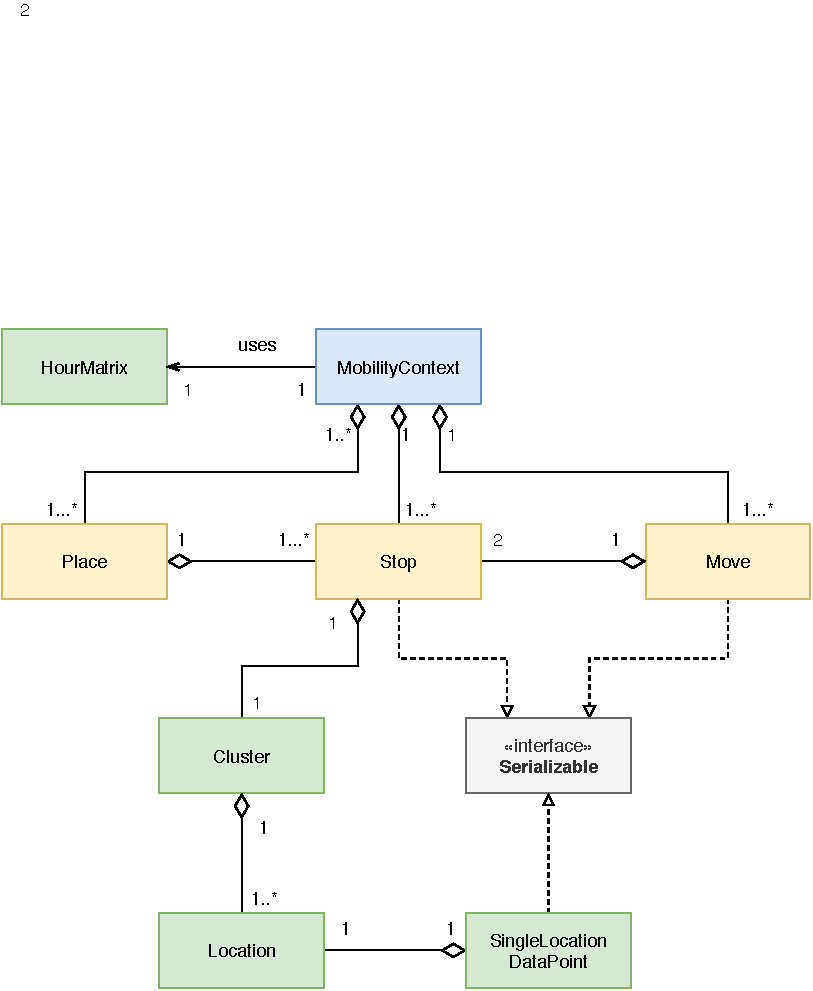
\includegraphics[width=\textwidth]{./images/uml-mobility-features.pdf}
    \caption{UML diagram for the classes used in the \textit{Mobility Features Package}.}
    \label{fig:my_label}
\end{figure}


